\section{Wikitty Struts}

Cette partie sur wikitty n'était pas prévu au départ, mais à l'utilisation
il s'est avéré que le dévellopement d'un tel module était nécessaire, et que
le travail précédement effectué sur la partie site de wikitty publication
pouvait rendre la tache plus rapide.


\subsection{Objectfifs}

L'édition de wikitty ou tout simplement l'utilisation de wikitty au sein de 
formulaire sont des éléments récurents dans les applications developpée 
chez code lutin, puisque en effet Wikitty est largement utilisé comme support
de base de donnée. 

L'objectif de ce module wikitty-struts à donc été de créer une taglib permettant
la génération des formulaires plus aisée pour les wikitty, afin de ne pas 
avoir à refaire ce que l'on a déjà fait pour une autre application.

Pour avoir une tag lib la plus complète possible il a été décidé d'en faire une
qui marcherait de la même façon que la taglib struts de base, et se reservirait
de ses méchanismes interne, avec les templates.

\subsection{La création d'un tag}

\begin{figure}[!ht]
  	%[height=12cm,width=15cm]
\centering
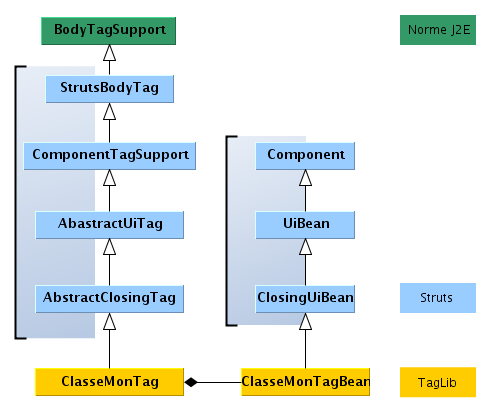
\includegraphics[height=7cm,width=9cm]{image/explicationTag.png}
  		\caption{Diagramme des tags avec struts}
  		\label{diagtagstruts}
\end{figure}

La création d'un tag classique, sans struts se fait par héritage de classe 
tel que "TagSupport" qui est une des classes défini dans la norme J2E pour la 
création des tags. En plus de la définition de la classe java, il faut écrire
dans un fichier xml (.tld) la définition du tag. La création de tag ainsi oblige
à écrire le code html directement dans le corps de la classe ou de devoir prévoir
l'architecture de support pour des templates.

Les templates permettent en fait de séparer le rendu du post traitement effectué
sur les attributs d'un tag, il permettent aussi de supporter plusieurs "thèmes", 
c'est à dire des collections de css pour changer le rendu, etc.

Faire des tag comme struts c'est un peu différent donc, sur la figure \ref{diagtagstruts} 
on voit qu'il y a une certaine architecture déjà mise en place. Il y a une chaine 
d'héritage étendant la norme pour les tag, et de l'autre une chaine d'héritage 
de classe spécifique à struts. 

Pour créer des tags spécifique on se place en bout de chaine, comme on le voit 
avec \emph{classeMontag} en héritant de \emph{AbstractClosingTag} on ne fait pas
grand chose, on délégue à la classe héritant de \emph{ClosingUiBean} qui contient 
elle la logique de traitement des éléments du tag. Ensuite il faut définir le
template écrit en \emph{freemarker}, qui lui contient le code html effectif 
qui sera écrit avec les éléments récupéré par la classe héritant de \emph{ClosingUiBean}.
Il faut aussi écrire le fichier tld pour la description.\\
\\
Pour résumer la création d'une taglib c'est:

\begin{itemize}
\item un fichier descripteur pour la taglib avec chaque tag de décrit 
\item une classe héritant de ClosingUiBean pour chaque tag
\item une classe héritant de AbstractClosingTag pour chaque tag qui délègue à son ClosingUiBean correspondant
\item des fichiers de template en freemarker pour chaque tag
\end{itemize}

%mettre un exemple de template ?


\subsection{La taglib wikitty struts "ws"}

Les tags ainsi developpé ont deux utilisations possible, la création d'un 
formulaire d'édition de wikitty, ou la création de formulaire utilisant les 
champs de wikitty comme champs. 

La différenciation de l'utilisation des tags passent par l'utilisation du tag 
de la taglib ws:form, qui implique que dans ce cas on se trouve dans l'édition d'un
wikitty.


A l'utilisation si on met seulement le tag \verb!ws:form! et la source de donné 
(le wikitty) un formulaire basic va être créé en fonction du type des champs
du wikitty, ensuite en utilisant les autres tag ou différent attribut du tag 
\verb!ws:form! il est possible de choisir d'exclure de l'édition des extensions,
des champs ou de choisir le type d'affichage pour un champ donné (et identifié
par son nom complet soit nomExtention.nomChamp).

En plus de fournir des tags pour la création de formulaire, la tag lib propose 
une action qui permet de prendre en compte les modifications de wikitty envoyé
par le formulaire. Il s'agit d'une action abstraite struts que l'utilisateur à 
besoin d'étendre pour implémenter la méthode accédant au proxy.

%utilisation des tags ? avec des exemples ou hje met tout en annexe  ?

%Présenter ici les différents tag rapidement avec les plus pertinent de façon plus 
%détaillés.





